\ifdefined\MAINDOC\else
\documentclass[10pt, a4paper, fleqn]{article}
\usepackage{base}

\begin{document}
    \title{Skript Mathe 2}
    \date{6. Mai 2018}
    \maketitle
\fi
    \begin{enumerate}[1., resume]
        \item Falls $(S_k)$ gegen $s \in \IR$ konvergiert, heißt die Reihe
        konvergent gegen s. Man schreibt:
        $$
            \lim_{k \to \infty} (S_k) = \lim_{k \to \infty} \qt{\sum_{i=1}^k a_i} = \sum_{i = 1}^\infty a_i = s
        $$
        Andernfalls heißt die Reihe divergent.
        
        \item Entsprechend kann man für eine Folge $(a_n)_{n \geq n_o}$ die Reihe
        $\sum_{i = n_o}^\infty a_i$ definieren.

        \item $\sum_{i=1}^\infty$ heißt absolut konvergent, falls $\sum_{i=1}^\infty \abs{a_i}$ konvergiert.
    \end{enumerate}

    \subsection{Bemerkung}
    Falls die Folgen der Partialsummen von $\sum_{i = n_o}^\infty a_i$ bestimmt gegen $+\infty (-\infty)$ divergiert,
    so schreiben wir: $\displaystyle\sum_{i = n_o}^\infty a_i = \infty (-\infty)$

    \subsection{Beispiele}
    \begin{enumerate}[a)]
        \item $\displaystyle\sum_{k=1}^\infty k = 1 + 2 + 3 + ... = \infty$
        \item \[\begin{aligned}
            &\underbrace{\sum_{k=1}^n (-1)^k}_{S_n} = \begin{cases}
                -1 &\text{n ungerade} \\
                1 &\text{n gerade}
            \end{cases} \\
            &\imp \sum_{k=1}^\infty (-1)^k \text{ divergent}
        \end{aligned}\]
        \item Harmonische Reihe $\displaystyle\sum_{k=1}^\infty \frac{1}{k}$ ist divergent.
        $$
            S_n = 1 + \frac{1}{2} +
            \underset{\hbox{$> 2 \cdot \frac{1}{4} = \frac{1}{2}$}}{\boxed{\frac{1}{3} + \frac{1}{4}}} +
            \underset{\hbox{$> 4 \cdot \frac{1}{8} = \frac{1}{2}$}}{\boxed{\frac{1}{5} + ... + \frac{1}{8}}} +
            \underset{\hbox{$> 8 \cdot \frac{1}{16} = \frac{1}{2}$}}{\boxed{\frac{1}{9} + ... + \frac{1}{16}}} + ... + \frac{1}{n}
        $$
        $\imp S_n > 1 + \frac{1}{2} + \frac{1}{2} + \frac{1}{2} + ...$

        Per Induktion: $S_{2^m} \geq 1 + \frac{m}{2} \xrightarrow[m \to \infty]{} \infty \imp (S_{2^m})$ divergent.
        \item $\displaystyle\sum_{k = 0}^\infty \frac{1}{2^k} = 1 + \frac{1}{2} + \frac{1}{4} + \frac{1}{8} + ...$ konvergent

        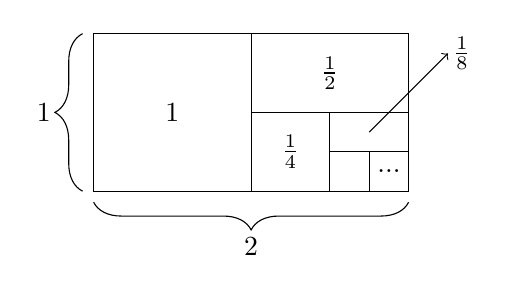
\begin{tikzpicture}[x = 2cm, y = 2cm]
            \draw (0, 0) rectangle ++(2, 1);
            \draw (1, 0) -- (1, 1) node[shift={(-0.5, -0.5)}] {1};
            \draw (1, 0.5) -- (2, 0.5) node[shift={(-0.5, 0.25)}] {$\frac{1}{2}$};
            \draw (1.5, 0) -- (1.5, 0.5) node[shift={(-0.25, -0.25)}] {$\frac{1}{4}$};
            \draw (1.5, 0.25) -- (2, 0.25);
            \draw[->] (1.75, 0.375) -- ++(0.5, 0.5) node[xshift = 5pt] {$\frac{1}{8}$};
            \draw (1.75, 0) -- (1.75, 0.25) node[shift={(0.125, -0.125)}]{...};

            \draw [decorate, decoration= {brace, amplitude = 10pt, raise = 4pt}, yshift = 0]
                (0, 0) -- (0, 1) node[midway, xshift = -18pt] {1};
            
                \draw [decorate, decoration= {brace, mirror, amplitude = 10pt, raise = 4pt}, yshift = 0]
                (0, 0) -- (2, 0) node[midway, yshift = -20pt] {2};
        \end{tikzpicture}

        und $\displaystyle \sum_{k=0}^\infty \frac{1}{2^k} = 2$

        \item \underline{Geometrische Reihe}

        Für $g \in \IR, |q| < 1$ gilt $\displaystyle\sum_{k=0}^\infty q^k = \frac{1}{1-q}$, \\
        denn $\displaystyle S_n = \sum_{k=0}^\infty q^k = \frac{1-q^{n+1}}{1-q}$ (Beweis mit vollständiger Induktion)

        Da $q^{n+1} \xrightarrow[n \to \infty]{} 0$ für $|q| < 1$ (1.10), folgt $S_n \to \dfrac{1}{1-q}$. \\
        Andererseits ist $\displaystyle\sum_{k=0}^\infty q^k$ divergent für $|q| \geq 1$ (2.9)

        \begin{itemize}
            \item In Beispiel d) is $q = \frac{1}{2}$ und $\displaystyle\sum_{k=0}^\infty \frac{1}{2^k} = \frac{1}{1 - \frac{1}{2}} = 2$
            \item $\displaystyle \sum_{k=0}^\infty \qt{-\frac{1}{2}}^k = \frac{1}{1 - \frac{1}{2}} = \frac{2}{3}$

            Diese Reihe ist sogar absolut konvergent.

            \item $\displaystyle \sum_{k=3}^\infty \qt{\frac{2}{3}}^k = \sum_{k=0}^\infty \qt{\frac{2}{3}}^{k+3}
                = \qt{\frac{2}{3}}^3 \cdot \sum_{k=0}^\infty \qt{\frac{2}{3}}^k 
                = \qt{\frac{2}{3}}^3 \cdot \underbrace{\frac{1}{1-\frac{2}{3}}}_{3} = \frac{8}{9}$
            
            \textbf{Achtung bei Index-Verschiebung!} %TODO: Warning symbol?
        \end{itemize}
    \end{enumerate}

    \subsection{Satz: Rechenregeln für Reihen}
    Gegeben seien zwei konvergente Reihen mit $\sum_{k=1}^\infty a_k = a, \sum_{k=1}^\infty b_k = b$ \\
    und $c \in \IR$.
    Dann gilt:
    \begin{enumerate}[a)]
        \item $\displaystyle \sum_{k=1}^\infty (a_k + b_k) = \sum_{k=1}^\infty (a_k) + \sum_{k=1}^\infty (b_k) = a + b$
        \item $\displaystyle \sum_{k=1}^\infty c - a_k = c \cdot \sum_{k=1}^\infty a_k = c \cdot a$
        
        Beweis folgt direkt aus 1.13.
    \end{enumerate}
    
    \subsection{Satz: Konvergenz und Divergenzkriterien für Reihen}

    Ist $(S_n)$ mit $S_n = \sum_{k=1}^\infty a_k$ nach oben beschränkt und $a_k > 0 \ \forall k \in \IN$, so ist
    $\sum_{k=1}^\infty a_k$ konvergent. (Folgt direkt aus 1.23)

    \subsection{Cauchy-Kriterium}
    $\sum_{i=1}^\infty a_i$ konvergiert $\eqv \ \forall \epsilon > 0 \ \exists N \in \IN:$
    \[\begin{aligned}
        \underbrace{\abs{a_n + ... + a_k}} < \epsilon \quad \forall k \geq n \geq N \\
        \Big[= \abs{S_k - S_{n - 1}} = \Big|\sum_{i=1}^k a_i - \sum_{i=1}^{n-1} a_i\Big|\Big]
    \end{aligned}\]
    (Folgt aus 1.40)

    \subsection{Satz: Absolute Konvergenz}
    Ist $\sum_{i=1}^\infty a_i$ absolut konvergent, so ist $\sum_{i=1}^\infty$ auch konvergent.

    \textbf{Beweis: } Sei $\epsilon > 0. \imp \ \exists N \in \IN$: $|a_n| + ... + |a_k| < \epsilon \quad \forall k \geq N$.

    Da $|a_n| + ... + |a_k| \leq |a_n| + ... + |a_k| < \epsilon \quad \forall k \geq n \geq N$, \\
    ist 2.6 für $\sum_{i=1}^\infty a_i$ erfüllt.

    \subsection{Korollar: Dreiecksungleichung für Reihen}

    Für jede absolut konvergente Reihe $\sum_{i=1}^\infty a_i$ gilt:
    $$
        \Big| \sum_{i=1}^\infty a_i \Big| \leq \sum_{i=1}^\infty a_i |a_i|
    $$

    \textbf{Beweis: } Sei $\sum_{i=1}^\infty a_i$ absolut konvergent. Dann:
    \[\begin{aligned}
        &\bullet \lim_{k \to \infty}(S_k) \underset{2.1}{=} \lim_{k \to \infty} \qt{\sum_{i=1}^K a_i} \\
        &\text{Da } \lim_{k \to \infty}|S_k| = \Big|\lim_{k \to \infty}\Big| \quad
        \left[\begin{array}{c}
            C_i \to c \\
            \imp |C_i| \to |c|
        \end{array} (1.13) \right], \\
        &\text{ist} \lim_{k \to \infty} \abs{\sum_{i=1}^k a_i} = \abs{\sum_{i=1}^\infty a_i} \ (*) \\
        &\bullet \lim_{k \to \infty} \qt{\sum_{i=1}^k |a_i|} \underset{2.1}{=} \sum_{i=1}^\infty |a_i| \ (**) 
    \end{aligned}\]
    \[\begin{aligned}
        \text{Insgesamt: } &\abs{\sum_{i=1}^k a_i} \leq \sum_{i=1}^k |a_i| \quad \Big| \lim_{k \to \infty} \\
        & \underset{(*),(**)}{\eqv} \abs{\sum_{i=1}^\infty a_i} \leq \sum_{i=1}^\infty |a_i| \quad \qed
    \end{aligned}\]

    \subsection{Satz: Divergenzkriterium}
    Ist $\sum_{i=1}^\infty a_i$ konvergent, so ist $(a_n)$ eine Nullfolge. \\
    D.h. Ist $(a_i)$ keine Nullfolge, so divergiert $\sum_{i=1}^\infty a_i$.

    \textbf{Beweis: } $\sum_{i=1}^\infty a_i$ konvergiert $\underset{2.6}{\imp} \ \forall \epsilon > 0 \ \exists N \in \IN:$

    $|a_n + ... + a_k| < \epsilon \ \forall k \geq n \geq N.$
    
    Wähle $k=1 \imp |a_n| < \epsilon \ \forall n \geq N \imp (a_n)$ Nullfolge. $\qed$

    \subsection{Majorantenkriterium}
    Seien $(a_n), (b_n)$ Folgen in $\IR$ mit $0 \leq a_n \leq b_n \quad \ n \in \IN$. \\
    Ist dann $\sum_{i=1}^\infty b_i$ konvergent, so ist auch $\sum_{i=1}^\infty a_i$ konvergent.

    \textbf{Beweis: } Sei $\epsilon > 0 \underset{2.6}{\imp} \ \exists N \in \IN: |a_n + ... + a_k|$
    
    $\underset{\mathclap{\overbrace{0 \leq a_1 \leq b_i \ \forall i}}}{\leq}|b_n + ... + b_k| < \epsilon \quad \forall k \geq n \geq N \qed$
\ifdefined\MAINDOC\else
\end{document}
\fi